\documentclass[master=elt,masteroption=eg,english]{kulemt}
\setup{title={The best master's thesis ever},
  author={Een Auteur\and Tweede Auteur},
  promotor={Prof.\,dr.\,ir.\ Weet Beter},
  assessor={Ir.\,W. Eetveel\and W. Eetrest},
  assistant={Ir.\ A.~Assistent \and D.~Vriend}}
% De volgende \setup mag verwijderd worden als geen fiche gewenst is.
\setup{filingcard,
  translatedtitle={Beste masterproef ooit al geschreven},
  udc=621.3,
  shortabstract={Hier komt een heel bondig abstract van hooguit 500
    woorden. \LaTeX\ commando's mogen hier gebruikt worden. Blanco lijnen
    (of het commando \texttt{\string\pa r}) zijn wel niet toegelaten!
    \endgraf \lipsum[2]}}
% Verwijder de "%" op de volgende lijn als je de kaft wil afdrukken
%\setup{coverpageonly}
% Verwijder de "%" op de volgende lijn als je enkel de eerste pagina's wil
% afdrukken en de rest bv. via Word aanmaken.
%\setup{frontpagesonly}

% Kies de fonts voor de gewone tekst, bv. Latin Modern
\setup{font=lm}

% Hier kun je dan nog andere pakketten laden of eigen definities voorzien

% Tenslotte wordt hyperref gebruikt voor pdf bestanden.
% Dit mag verwijderd worden voor de af te drukken versie.
\usepackage[pdfusetitle,colorlinks,plainpages=false]{hyperref}

%%%%%%%
% Om wat tekst te genereren wordt hier het lipsum pakket gebruikt.
% Bij een echte masterproef heb je dit natuurlijk nooit nodig!
\IfFileExists{lipsum.sty}%
 {\usepackage{lipsum}\setlipsumdefault{11-13}}%
 {\newcommand{\lipsum}[1][11-13]{\par Hier komt wat tekst: lipsum ##1.\par}}
%%%%%%%

%\includeonly{chap-n}
\begin{document}

\begin{preface}
  I would like to thank everybody who kept me busy the last year,
  especially my promoter and my assistants. I would also like to thank the
  jury for reading the text. My sincere gratitude also goes to my wive and
  the rest of my family.
\end{preface}

\tableofcontents*

\begin{abstract}
  The \texttt{abstract} environment contains a more extensive overview of
  the work. But it should be limited to one page.

  \lipsum[1]
\end{abstract}

\begin{abstract*}
  In dit \texttt{abstract} environment wordt een al dan niet uitgebreide
  Nederlandse samenvatting van het werk gegeven.
  Wanneer de tekst voor een Nederlandstalige master in het Engels wordt
  geschreven, wordt hier normaal een uitgebreide samenvatting verwacht,
  bijvoorbeeld een tiental bladzijden. 

  \lipsum[1]
\end{abstract*}

% Een lijst van figuren en tabellen is optioneel
%\listoffigures
%\listoftables
% Bij een beperkt aantal figuren en tabellen gebruik je liever het volgende:
\listoffiguresandtables
% De lijst van symbolen is eveneens optioneel.
% Deze lijst moet wel manueel aangemaakt worden, bv. als volgt:
\chapter{List of Abbreviations and Symbols}
\section*{Abbreviations}
\begin{flushleft}
  \renewcommand{\arraystretch}{1.1}
  \begin{tabularx}{\textwidth}{@{}p{12mm}X@{}}
    LoG   & Laplacian-of-Gaussian \\
    MSE   & Mean Square error \\
    PSNR  & Peak Signal-to-Noise ratio \\
  \end{tabularx}
\end{flushleft}
\section*{Symbols}
\begin{flushleft}
  \renewcommand{\arraystretch}{1.1}
  \begin{tabularx}{\textwidth}{@{}p{12mm}X@{}}
    42    & ``The Answer to the Ultimate Question of Life, the Universe,
            and Everything'' according to \cite{h2g2} \\
    $c$   & Speed of light \\
    $E$   & Energy \\
    $m$   & Mass \\
    $\pi$ & The number pi \\
  \end{tabularx}
\end{flushleft}

% Nu begint de eigenlijke tekst
\mainmatter

\chapter{Introduction}
\label{cha:intro}

%\epigraph{\textit{``If we want machines to think, we need to teach them to see.''}}{\textit{- Li Fei-Fei}}

%% shurong: replace this part (til the end of 1.1) by some introductions on image-text alignment and cross modal retrieval

As a part of the millions of internet users who often surf on the internet, we always ``Google'': enter the keywords to be searched to retrieve our desired text information, which is to retrieve text with text in this case. Sometimes we also upload images on Google to find similar ones, which refers to using an image to retrieve images. However, considering the situation when we use textual information to retrieve images on Google, at this time the type of information we enter and the type of information obtained is different, known as ``cross modal''.

Cross modal retrieval can be understood as finding the relationship between different modal samples and using a particular modal sample to search for other modal samples with approximate semantics. For example: use the image to retrieve the corresponding text, or use the text to retrieve the desired image. Of course, modals are not limited to images and text, such as voice, physiological signals, and video can be used as components of cross modal retrieval.

The goal of cross modal retrieval is to calculate the similarity between different modal data. For a given query sample, retrieve different modal data related to the query sample. The key challenge lies in the inconsistent representation of different modalities, making it difficult to directly measure the similarity, that is, the ``semantic gap'' problem. There are two mainstream cross-modal retrieval methods: common space learning methods and cross-modal similarity measurement methods.

The common space learning method enables a cross-modal similarity to be directly measured in this space by learning a unified common space for different modal data, mainly including traditional statistical association analysis methods, deep learning based methods, graph-based reduction Methods, metric learning methods, ranking learning methods, dictionary learning methods, cross modal hashing methods, etc.

The cross modal similarity measurement method does not learn the common space, but directly calculates the cross modal similarity, mainly including graph-based methods and nearest neighbour analysis methods. Besides, there are some other cross modal retrieval methods, such as correlation feedback analysis method, multi-modal theme model method, etc.

At present, the types of multimedia in cross modal retrieval mainly include images, text, voice, video and 3D graphics. Most cross modal retrieval methods are currently limited to the use of images and text, as well as a small number of other types of voice and video. On the one hand, almost no databases are containing these five modal types; on the other hand, there are ``semantic gaps'' in the various forms of different modal types.

The ``semantic gap'' problem is a core challenge faced by cross-modal retrieval: data of different modalities have different feature representations, and their similarity is difficult to measure directly. In order to solve the above problem, an intuitive method is to unify the representation across modalities, that is, to map different modal data from their independent representation spaces into a third-party, public space so that they can measure the similarity of each other. In recent years, with the rapid development and broad application of deep learning, the unified representation method based on deep learning has become a research hot spot and mainstream.

%As the most basic and influential part of human's sensory nervous system, vision plays a vital part in all kinds of recognition tasks. A glance at an image is sufficient for a human to point out and describe an immense amount of details about the visual scene. Traditionally, object recognition and description were performed manually. As time passed, the number of images in many systems grew to more substantial than terabyte size, and could no longer be maintained manually, which brought the idea of machine learning and computer vision also formed a part of artificial intelligence. 

%The process of ``teaching machines to see'' has been widely discussed since the late 20$^{th}$ century and focused on modelling the 3D shape of objects. The latter focus emphasises the identification of objects, and this was achieved by adopting the AdaBoost \cite{adaboost} algorithm. Recently, since neural network-based algorithm AlexNet \cite{alexnet} won the object recognition ImageNet \cite{imagenet} competition in 2012, the field of computer vision began to make breakthroughs. At present, the top technology in the field of computer vision has been continuously approaching human performance. Besides, the learning mechanism, performance and security of neural networks are discussed in more depth.

%\section{Computer Vision}

%Computer vision (CV) refers to the ability of machines to perceive the environment, and it is the subject of researching machine vision capabilities, or the subject that enables machines to analyse the environment and the stimuli therein visually. Machine vision usually involves the evaluation of images or videos. The British Machine Vision Association (BMVA) defines machine vision as "the automatic extraction, analysis, and understanding of useful information from a single image or a series of images." \cite{bmva}

%A real understanding of our environment is not achievable only by visual representation. More precisely, it is the process of transmitting visual cues to the primary visual cortex through the optic nerve, and then being analysed by the brain in a highly characterised form. Extracting explanations from this sensory information contains almost all of our natural evolution and subject experience, that is, how evolution survives us, and how we learn and understand the world in our lifetime.

%In this respect, the visual process is only the process of transmitting images and interpreting them. However, from a computational point of view, the images are closer to thought or cognition and involve many functions of the brain. Therefore, due to the remarkable cross-domain characteristics, many people think that computer vision is a real understanding of the visual environment and its context, and will lead us to achieve reliable artificial intelligence.

\section{Motivation}
%% shurong: extend the motivation in the abstract and emphasize that image-text alignment in the cultural heritage domain has not been a lot exploit yet, they are quite popular for natural images. you can also merge this part with the above part if the content is too less
Image-text alignment is a fundamental research topic in the inter-field of computer vision and natural language processing. It includes two sub-tasks: image annotation and image search. The topic of image-text alignment and cross modal retrieval has been widely discussed in the field of natural images. However, image-text alignment in the cultural heritage domain has not been a lot exploit yet. It can save the intense labour from annotating the artworks for online digital artwork archives if we can automatically describe an artwork image or sub-image with its textual attributes. Furthermore, this topic can help to boost the multi-modal question answering performance in the cultural heritage domain by providing fine-grained image-text correspondence information \cite{mqa}. Therefore, it is interesting to explore the methods that can figure out the artwork image or sub-image and text correspondence.

While a large number of papers discussed aligning image-text and coarse-grained modal information retrieval, the fragment level image-text alignment problem has not been as widely dealt within the multi-modal question-answering research domain. Coarse-grained modal information retrieval can retrieve information between image and text. However, it usually does not work well on artwork datasets which usually contain some fine-grained patterns and objects in one artwork image, therefore reduce the effectiveness of the retrieval model. In this section, we look at two simple examples of ancient Egyptian artworks and how textual description can be generated to match its image.

\begin{figure}[h!]
\centering
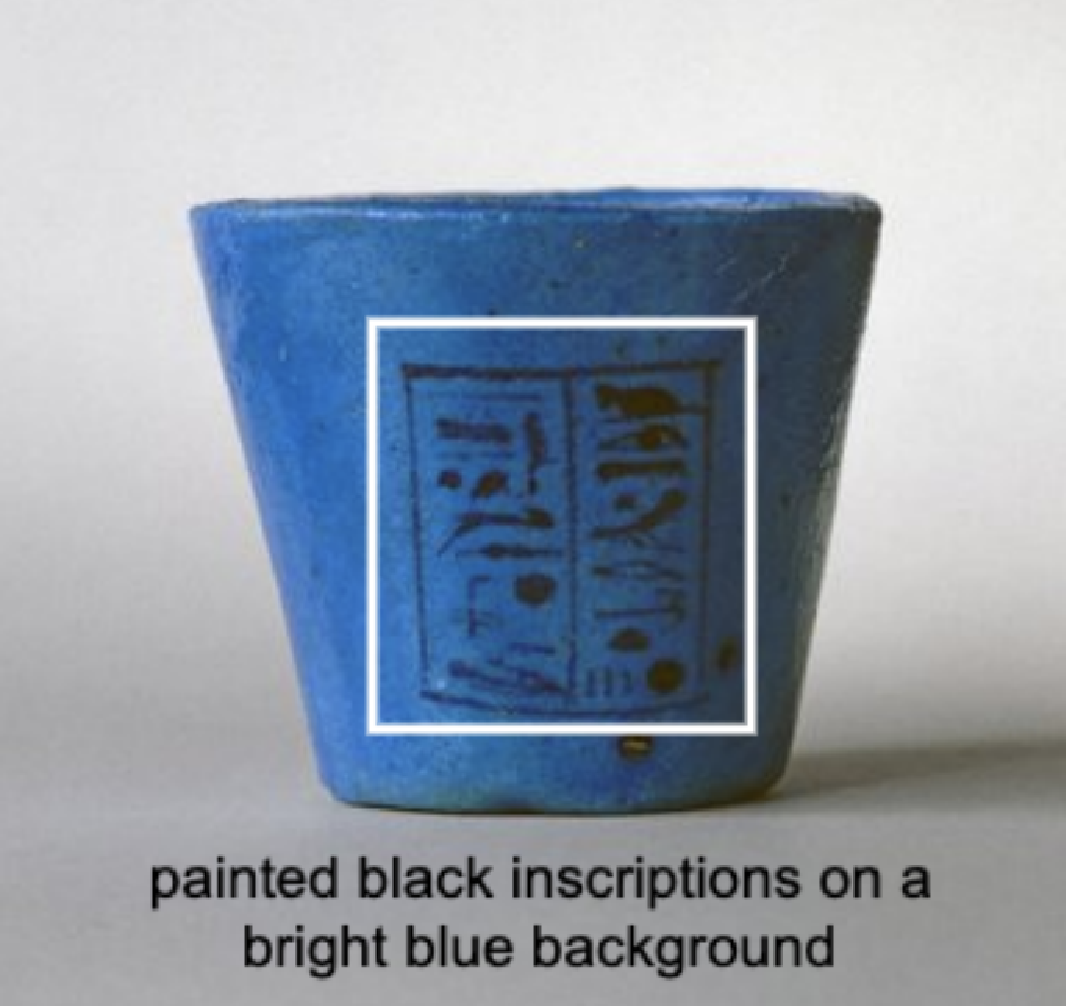
\includegraphics[width=0.35\textwidth]{artwork_fine1.pdf}
\caption{Ancient Egyptian Artwork Example (coarse-grained)}
\label{fig:artwork1}
\end{figure}

Figure \ref{fig:artwork1} shows a small blue container with black inked motifs on it. Using a coarse-grained multi-modal retrieval model, we can generate the textual description ``\textit{painted black inscriptions on a bright blue background}'', which is sufficient enough for this artwork. However, in the real-world scenarios, there is much more likely for us to encounter an artwork showing in Figure \ref{fig:artwork2}. Our traditional coarse-grained multi-modal retrieval model generates ``\textit{a red and a white pot}'' for this artwork but it is not detailed and did not cover sufficient information in the artwork image. Therefore, this motivated us to propose a fine-grained multi-modal retrieval model which can focus on the fragment level image/sentence retrieval. The description on the image was generated by our fine-grained multi-modal retrieval model, which has significantly more detailed information.

\begin{figure}[h!]
\centering
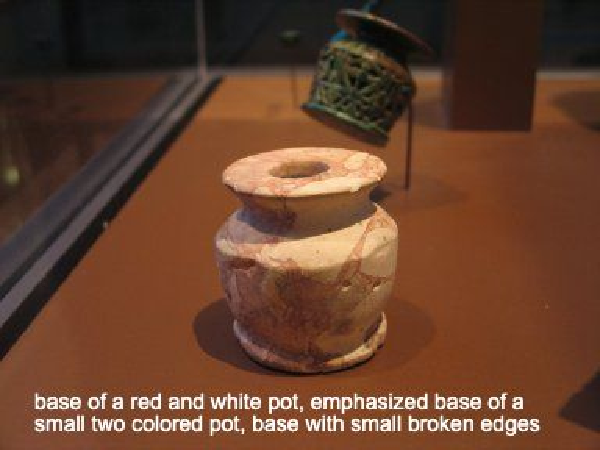
\includegraphics[width=0.45\textwidth]{artwork_fine2.pdf}
\caption{Ancient Egyptian Artwork Example (fine-grained)}
\label{fig:artwork2}
\end{figure}


%% shurong: move the examples in 1.2 to the dataset part. There are also redundant info in this section. double check and remove repeated content
\section{Dataset}

The datasets \cite{artworkcaption} involved in this thesis research are collected from the following online sources: the Brooklyn Museum \cite{brooklynmuseum}, the Metropolitan Museum \cite{themet}, and the British Museum \cite{thebritishmuseum}. Based on these sources, we have created two artwork datasets: the ancient Egyptian art image dataset and the ancient Chinese art image dataset. The two datasets are collected based on the geographical location of the origin of the artworks because caption words may differ much depending on the cultural background of the location. Detailed statistics of the two datasets are shown in Table \ref{fig:datasetstats}. 

\begin{table}[h!]
\centering
\begin{tabular}{|c|c|c|c|}
\hline
\textbf{Dataset}          & \textbf{Num. of Artworks} & \textbf{Aver. Length} & \textbf{Num. of Tokens} \\ \hline
\textbf{Egyptian} & 16,146                       & 9                       & 10,694                     \\ \hline
\textbf{Chinese}  & 6,847                        & 10                      & 4,721                      \\ \hline
\end{tabular}
\caption{Statistics of Our Datasets \cite{artworkcaption}}
\label{fig:datasetstats}
\end{table}

The datasets have 22,993 high-quality artwork images recorded
in a controlled setting. Images are stored at varying dpi and the
compressed \verb|jpeg| image file size ranges between 20-300 KB. The paragraph-level descriptions are split into multiple sentences and a maximum of five sentences are retained for each artwork to reduce data imbalance. In addition, we removed noisy texts from the captions following a specific pattern, e.g, ``See 13.26.59'' \cite{artworkcaption}. The number is the accession number of an artifact that obviously cannot be derived from the input image or artwork type. We also remove duplicate images in the captioning datasets based on their hash code. Tokens occurring less than two times are removed from the training vocabulary. The datasets are all split into an 80\%, 10\%, and 10\% partition for respectively training, validation, and test.

Each artwork image has a corresponding record saved in a \verb|json| file containing their processed caption textual data. However, in our research, instead of using the original captions in the \verb|json| file, we extracted noun phrases from them and performed our alignment tasks between these noun phrases and images.

Here we focus on ancient Egyptian and Chinese artworks; we manually construct our datasets; they consist of 16,146 images from Egyptian domain and 6,847 images in Chinese. Figure \ref{fig:sampleEgyptian} and Figure \ref{fig:sampleChinese} show three examples of artworks from the Egyptian and Chinese collection with textual captions.

\begin{figure}[h!]
\centering
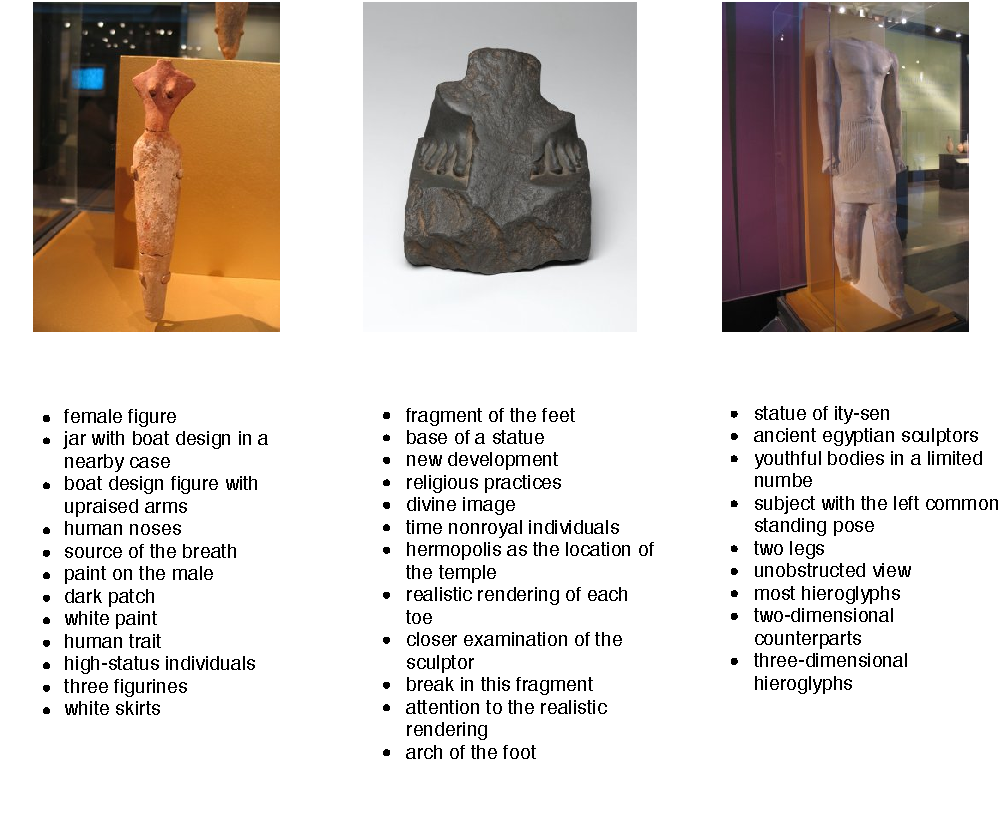
\includegraphics[width=0.9\textwidth]{egyptian.pdf}
\caption{Examples of Artworks of Egyptian Artwork Dataset}
\label{fig:sampleEgyptian}
\end{figure}

\begin{figure}[h!]
\centering
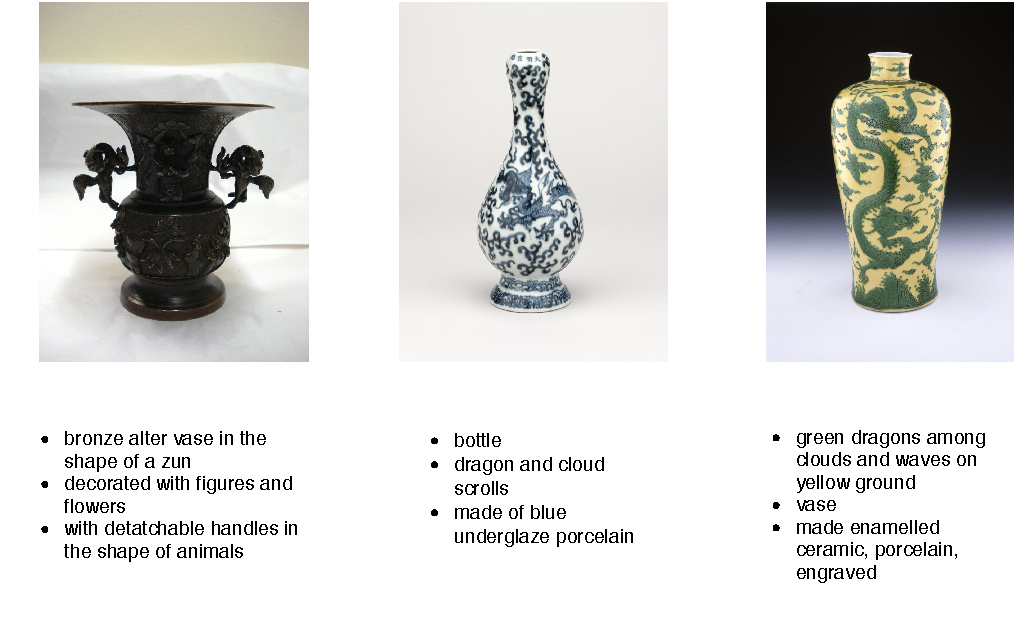
\includegraphics[width=\textwidth]{chinese.pdf}
\caption{Examples of Artworks of Chinese Artwork Dataset}
\label{fig:sampleChinese}
\end{figure}

\section{Research Questions}

In this thesis, we study fine-grained image-text alignment for artworks. Fine-grained image-text alignment refers to the fragment level cross modal (between image and text) retrieval. The prior sections list the background and motivations, the specific research questions that we look at are:

%% two research questions: 1. is the alignment model experimented on natural images effective for artwork items 2. can coarse-grained cross-modal retrieval modal be adapted to fine-grained retrieval and how?
\begin{itemize}
    \item Why mainstream coarse-grained image-text alignment techniques does not suit artwork domains well?
    \item Can we propose a practical approach that facilitates the textual attributes annotation of artwork images accurately and efficiently?
    \item Can we develop a fine-grained image-text alignment technique that can retrieve text from images and vice versa on fragment level?
\end{itemize}

\subsection{Cross Modal Retrieval Framework}

As mentioned above, our primary research task here is to achieve cross modal retrieval (i.e. between image and text) for artworks. Figure \ref{fig:framework} illustrates a brief working framework for the tasks.

%% [solved]shurong: the training data is a bit confusing. an image should be composed of a certain number of image fragments and the text is noun-phrase composed sentence .Or the picture can be kept here but you explain the two levels of retrieval clearly or even give examples.
\begin{figure}[h!]
\centering
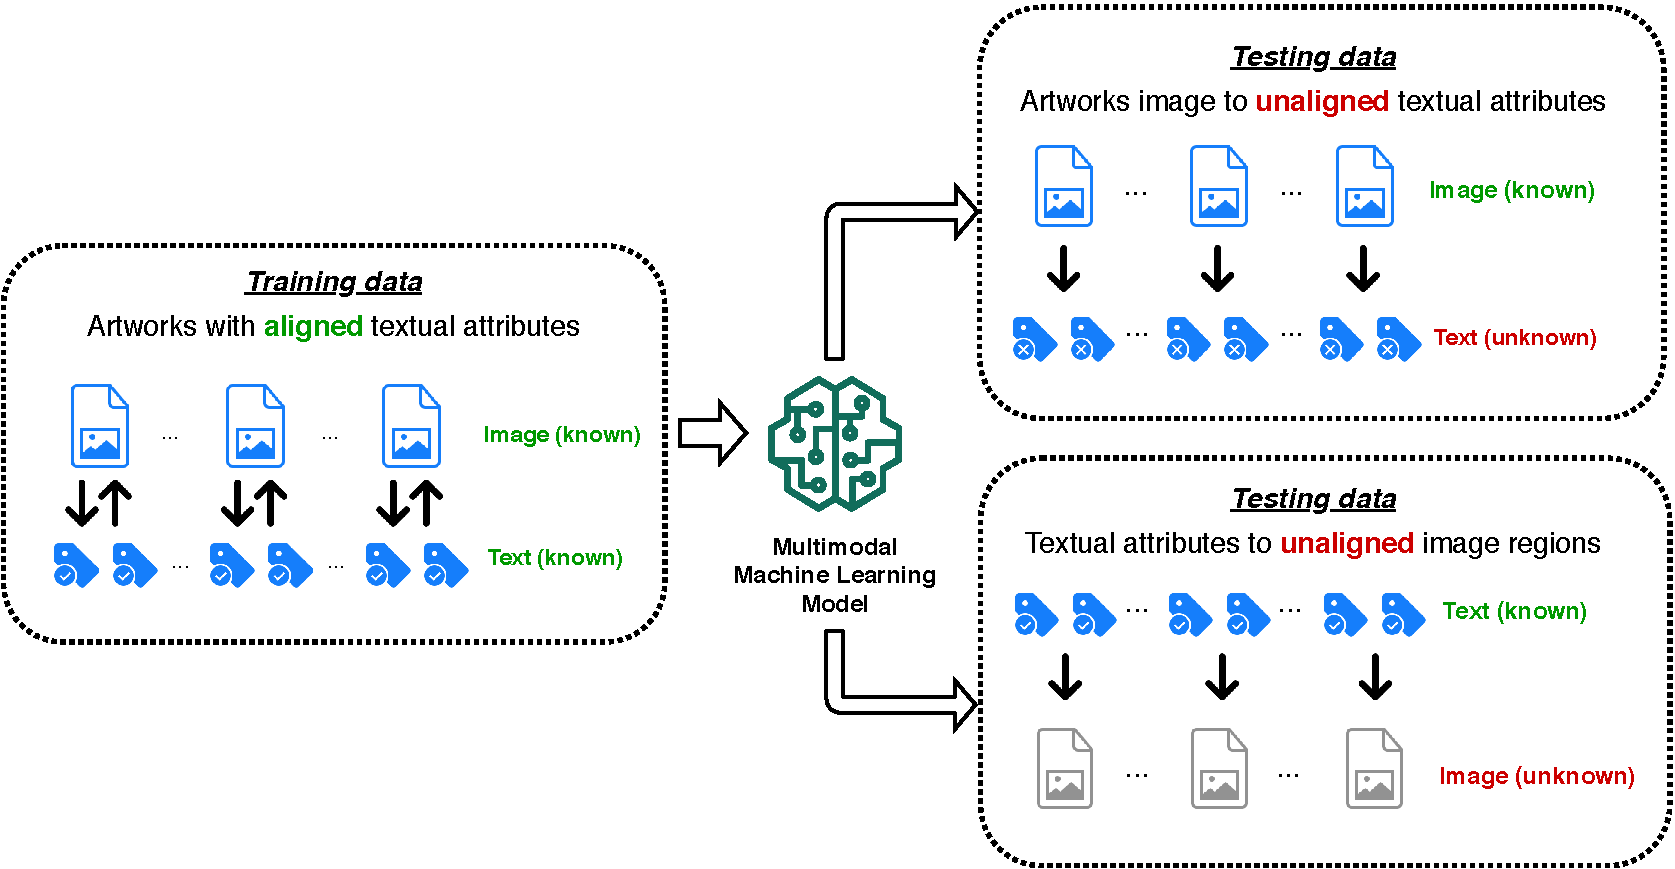
\includegraphics[width=\textwidth]{framework.pdf}
\caption{Cross Modal Retrieval Process}
\label{fig:framework}
\end{figure}

We train our multi-modal machine learning model on the known image features and corresponding textual attributes; this training process helps us learn the potential relationships between image and text. This trained model will be used to generate textual attributes from known image features and vice versa. We believe this may help with automating the artwork annotation process and significantly save labours on artworks classifications and searches.


\section{Contributions}
The main contributions made by this thesis are:

\begin{enumerate}
    \item We review work from several disciplines which may be of relevance to the present subject of inquiry and provide commentary on how the findings from these disciplines may be useful. (Section~\ref{cha:relatedworks})
    \item We adopted SCAN \cite{scan} as the coarse-grained cross modal retrieval model, analysed its structure and applied it on our proposed Egyptian and Chinese artworks datasets to achieve the image-text alignment. By employing this model, we are able to have a coarse-grained alignment between artworks image and textual attributes. This lays the foundation of our improved fine-grained model. (Section~\ref{cha:scan})
    \item By focusing on fragment level image features and textual attributes instead of feeding the whole images and sentences, we are able to perform cross modal retrieval in a more fine-grained level. This allows the future multi-modal retrieval tasks on artworks to achieve more accurate and stable results. (Section~\ref{cha:Method})
\end{enumerate}


\section{Structure of Thesis}

This thesis is structured into the following chapters:

\begin{itemize}
    
    \item \textit{Section~\ref{cha:intro} Introduction}\newline
    We provide the reader with a relevant background to understand this thesis.

    \item \textit{Section~\ref{cha:relatedworks} Related Works}\newline
    We introduce relevant research in image recognition, deep learning, object detection, natural language processing and image-text alignment. In particular, we detail seminal research and review the overall state of the current research. We also review the difference in the works pertaining to the traditional visual-semantic alignment technique versus the more recent cross attention image-text alignment framework.
    
    \item \textit{Section~\ref{cha:scan} Coarse-grained Cross Modal Retrieval}\newline
    We introduce our coarse-grained cross-modal retrieval modal - SCAN, discuss how its components interact with each other and explain how SCAN uses cross attention to improve image-text alignment. We also show the preliminary result running SCAN on our ancient Egyptian and Chinese artwork datasets.
    
    \item \textit{Section~\ref{cha:Method} Fine-grained Cross Modal Retrieval}\newline
    We proposed our improved fine-grained cross modal retrieval model, which now focus more on the fragment level image-text alignment. We then perform several experiments on evaluating the effectiveness of our image generation from text and vice versa by the recall. We also point out the direction of possible future improvements by discussing several recent related publications.
    
    \item \textit{Section~\ref{cha:conclusion} Conclusion}\newline
    We conclude the work and add some final reflections and remarks.
\end{itemize}
%%% Local Variables: 
%%% mode: latex
%%% TeX-master: "thesis"
%%% End: 

\include{chap-1}
\include{chap-2}
% ... en zo verder tot
\include{chap-n}
\chapter{Conclusion}
\label{cha:conclusion}
The final chapter contains the overall conclusion. It also contains
suggestions for future work and industrial applications.

\lipsum[1-7]

%%% Local Variables: 
%%% mode: latex
%%% TeX-master: "thesis"
%%% End: 


% Indien er bijlagen zijn:
\appendixpage*          % indien gewenst
\appendix
\chapter{Implementation Details}
\label{app:A}
This appendix provides some \verb|Python| source code for the implementation mentioned in Section \ref{cha:Method}.

\section{Project Structure}
In this section, we go through the structure of my implementation using structured tables. This gives the audience and future researchers a brief idea on how the process looks like.


\begin{table}[h!]
\centering
\begin{tabular}{|l|l|}
\hline
\multicolumn{1}{|c|}{Source Code File} & \multicolumn{1}{c|}{Description}  \\ \hline
\verb|egyptian_convert.py|             & \begin{tabular}[c]{@{}l@{}}Contains \verb|xml| parser and \verb|json| parser. \\ This generates caption for each picture, \\ extract features base on the corresponding \\ caption and also generate features for each \\ image by using parsed \verb|xml| file\end{tabular} \\ \hline
\verb|preprocess.ipynb|                 & \begin{tabular}[c]{@{}l@{}}Combines the features extracted from \\ botton-up attention (Egyptian)\end{tabular}                                                                                                                                          \\ \hline
\verb|chinese_artworks_convert.ipynb| & \begin{tabular}[c]{@{}l@{}}Combines the features extracted from \\ botton-up attention (Chinese)\end{tabular}                                                                                                                                           \\ \hline
\end{tabular}
\label{table:preprocesspython}
\caption{Python Source Code Files for Preprocessing}
\end{table}


%%%%%%%%%%%%%%

\begin{table}[h!]
\centering
\begin{tabular}{|l|l|}
\hline
\multicolumn{1}{|c|}{Source Code File} & \multicolumn{1}{c|}{Description}                                                                                                                             \\ \hline
\verb|data.py|                                & \begin{tabular}[c]{@{}l@{}}Class \verb|PrecompDataset| is where we changed\\ the path of extracted phrases and also where\\ to change process methods.\end{tabular} \\ \hline
\verb|model.py|                               & Provides SCAN model based on VSE++.                                                                                                                           \\ \hline
\verb|train.py|                               & \begin{tabular}[c]{@{}l@{}}Provides training process using settings in\\ \verb|model.py|.\end{tabular}                                                               \\ \hline
\end{tabular}
\label{table:trainpython}
\caption{Python Source Code Files for Training}
\end{table}



%%%%%%%%%%%%%%%

\begin{table}[h!]
\centering
\begin{tabular}{|l|l|}
\hline
\multicolumn{1}{|c|}{Source Code File} & \multicolumn{1}{c|}{Description}                                                                                          \\ \hline
\verb|evaluation.py|                          & \begin{tabular}[c]{@{}l@{}}Provides testing process using the fragment\\ level annotations and ground truth.\end{tabular} \\ \hline
\verb|demo.ipynb|                             & Provides a demo for testing process.                                                                                      \\ \hline
\end{tabular}
\label{table:testpython}
\caption{Python Source Code Files for Testing}
\end{table}


\subsection{Obtain Image Features}
We used bottom-up attention \cite{bottomup} to extract features from our Egyptian and Chinese artwork images. This methodolgy used a faster R-CNN and a ResNet101 as core architecture. We obtained a pre-trained model from its \href{https://github.com/peteanderson80/bottom-up-attention}{Github} open repository which was trained on \verb|VisualGenome| dataset consisting a large amount of real-world images. A sample image feature extraction command for Egyptian training images is displayed below:

\begin{lstlisting}
$ python bottom-up-features/extract_features.py 
--image_dir artworks/train --out_dir artworks/features 
--cfg bottom-up-features/cfgs/faster_rcnn_resnet101.yml 
--model bottom-up-features/models/bottomup_pretrained_10_100.pth
\end{lstlisting}

We save these obtained image features under \verb|/features| directory. These image features of Egyptian and Chinese artworks are available in numpy array format, which can be used for training directly in the future.

\subsection{Obtain Textual Features}

According to captions and corresponding image labels, we can extract the corresponding image names from \verb|xml| and \verb|json| files which contains textual attributes. This extraction process can be done using \verb|egyptian_convert.py|, \verb|python| script then generates captions for each image, make sure that each has a corresponding \verb|.txt| file created. These produced \verb|.txt| files are saved in \verb|/phrase| directory. 

To achieve the retrieval on a fragment level, we then extract noun phrases from these \verb|.txt| files. We use \verb|/preprocess.ipynb| to obtain \verb|vocab.json|. The API adopted here was proposed by Handler et al. \cite{nounphrase} and available on \href{https://github.com/slanglab/phrasemachine}{Github} as well.

\subsection{Training and Testing}
For training process, we can simply modify the \verb|PrecompDataset| class in \verb|data.py| to change related processing methods. A sample training command for Chinese training images is displayed below (with i-t average pooling formulation):

\begin{lstlisting}
python train.py --data_name chinese_artworks 
--logger_name $RUN_PATH/chinese_artworks_scan/log 
--model_name $RUN_PATH/chinese_artworks_scan/log 
--max_violation --bi_gru --img_dim 2048
--agg_func=Mean --cross_attn=i2t --lambda_softmax=4
\end{lstlisting}

For testing process, we load our saved model then run \verb|evaluation.py| script. A sample evaluation command is shown below:

\begin{lstlisting}[language=python]
from vocab import Vocabulary
import evaluation
evaluation.evalrank("$RUN_PATH/chinese_artworks_scan/model_best.pth.tar", data_path="$DATA_PATH", split="test")
\end{lstlisting}


%%%%%%%%%%%%%%

\section{Python Snippets}
In this section, we briefly display the preprocessing part of our implementation which is also crucial to the entire project as an efficient and accuracy extraction from \verb|xml| files can make the training and testing process easier and more smooth.

Here we focus on two specific files, one is \verb|egyptian_convert.py| which is able to parse \verb|xml| and \verb|json| files. Another one is \verb|preprocess.ipynb| which combines features and vocabularies for each distinct artwork.


\subsection{Texual Attribute Parser}

Here the code snippet of \verb|egyptian_convert.py| is displayed below. Similarly, \verb|chinese_artwork_convert.py| works for Chinese artwork dataset.

\begin{lstlisting}[language=Python]
import xml.etree.ElementTree as ET
import os
import numpy as np
from tqdm import tqdm
import json

# this module used to generate caption for each picture and extract features base on the corresponding caption

# parse the xml and get the text for relevant element

def get_text(path):
    tree = ET.parse(path)
    root = tree.getroot()
    file_name = root[1].text
    res = []
    for object in tree.findall("object"):
        res.append(object[0].text)
    return file_name,res

# generate features for each image by using parsed xml file

def xml_parser(path,features_path,save_path):
    list_dir = os.listdir(path)
    features = []
    not_list = []
    for image in tqdm(list_dir):
        file_path = os.path.join(features_path, image.split('.')[0] + '.npy')
        feature = np.load(file_path, allow_pickle=True).tolist()["features"]
        print(feature)
        feature = np.array(feature)
        features.append(feature[:10, :])
    features = np.stack(features)
    np.save(save_path, features)
    
def json_parser(path):

    # load the json files extract the sentence and corresponding picture name.
    
    with open(path,"r") as file:
        data = json.load(file)
        for image in data["images"]:
            try:
                file_name = image["filename"]+".txt"
                sentence = image["sentences"]
                sentence = sentence[0]["raw"]
            except:
                continue
            # save the sentence in relevant files
            with open(os.path.join("../data/phrase_train", file_name),"w") as f:
                f.write(sentence)
                
\end{lstlisting}

\subsection{Feature Combination}
Here the code snippet of \verb|preprocess.ipynb| is displayed below.

\begin{lstlisting}[language=Python]
import torchvision
import torch
import json
import cv2
import os.path as osp
from PIL import Image
from tqdm import tqdm_notebook
import numpy as np
import nltk
from collections import Counter

# combine the features extracted from botton-up attention

content = json.load(open(osp.join(dataset_name, 'caption_data.json')))

images = {
    'train': [],
    'test': [],
    'val': []
}

for image in content['images']:
    filepath = image['filepath']
    if len(image['sentences']) == 0:
        continue
    images[filepath].append(image)
    
for phase in images.keys():
    features = []
    for image in tqdm_notebook(images[phase]):
        file_path = osp.join(dataset_name, 'features', image['filename'].split('.')[0] + '.npy')
        print(file_path)
        feature = np.load(file_path)
        features.append(feature[:10, :])
    features = np.stack(features)
    np.save(osp.join(dataset_name, phase), features)

from vocab import Vocabulary, serialize_vocab
from collections import Counter
import phrasemachine

threshold = 4
counter = {}
for phase in images.keys():
    captions = [x['sentences'][0]['raw'] for x in images[phase]]
    for caption in captions:
        temp = list(phrasemachine.get_phrases(caption)["counts"].keys())
        for key in temp:
            if key not in counter.keys():
                counter[key] = 1
            else:
                counter[key] += 1
# Discard if the occurrence of the word is less than min_word_cnt.
words = [word for word, cnt in counter.items() if cnt >= threshold]

# create a vocab wrapper and add some special tokens
vocab = Vocabulary()
vocab.add_word('<pad>')
vocab.add_word('<start>')
vocab.add_word('<end>')
vocab.add_word('<unk>')

# Add words to the vocabulary.
for i, word in enumerate(words):
    vocab.add_word(word)
serialize_vocab(vocab, osp.join(dataset_name, 'vocab.json'))

with open(osp.join(dataset_name, 'data.json'), 'w') as f:
    json.dump(images, f)
\end{lstlisting}


%%% Local Variables: 
%%% mode: latex
%%% TeX-master: "thesis"
%%% End: 

% ... en zo verder tot
\chapter{Experiment Details}
\label{app:n}
details

\section{Training Settings}



%%% Local Variables: 
%%% mode: latex
%%% TeX-master: "thesis"
%%% End: 


\backmatter
% Na de bijlagen plaatst men nog de bibliografie.
% Je kan de  standaard "abbrv" bibliografiestijl vervangen door een andere.
\bibliographystyle{abbrv}
\bibliography{references}

\end{document}

%%% Local Variables: 
%%% mode: latex
%%% TeX-master: t
%%% End: 
